\DiaryEntry{Integrating $1/(x^4 - x^2+1)$}{2022-02-14}{Integrals}

Taken from \href{https://math.stackexchange.com/questions/4367988/how-to-find-exact-value-of-integral-int-0-infty-frac1-leftx4-x2}{here}.

We want to calculate the following integral,

\bee
I(1) = \int_0^\infty \frac{dx}{x^4 - x^2 + 1}
\eee

We first make the substitution $u = \frac{1}{x}$ with $du/dx = -1/x^2 \rightarrow dx = -x^2 du = - du/u^2$ and obtain

\bee
I(1) = - \int_\infty^0 \frac{du/u^2}{1/u^4 - 1/u^2 + 1} = \int_0^\infty \frac{du/u^2}{1/u^4 - 1/u^2 + 1} = \int_0^\infty \frac{u^2 du}{u^4 - u^2 + 1}
\eee

where we multiplied numerator and denumerator with $u^4$ in the last equation. At first sight we have not gained anything, but we can combine the two integrals as

\bee
I(1) = \frac{1}{2} \int_0^\infty \frac{x^2+1 dx}{x^4 - x^2 + 1}
\eee

We can rewrite this further

\bee
I(1) = \frac{1}{2} \int_0^\infty \frac{1 + 1/x^2 dx}{x^2 - 1 + 1/x^2} = \frac{1}{2} \int_0^\infty \frac{1 + 1/x^2 dx}{(x - 1/x)^2 + 1}
\eee

and substitute $u = x-\frac{1}{x}$ with $\frac{du}{dx} = 1+\frac{1}{x^2} \rightarrow dx = \frac{du}{1 + \frac{1}{x^2}}$ and therefore

\bee
I(1) = \frac{1}{2} \int \frac{1 + \frac{1}{x^2}}{u^2 + 1} \frac{du}{1 + \frac{1}{x^2}} = \frac{1}{2} \int \frac{du}{1+u^2} = \frac{1}{2} \arctan(u) = \frac{1}{2} \left. \arctan\left(x - \frac{1}{x}\right) \right|_0^\infty = \frac{\pi}{2} \qed
\eee

The following Figure shows the two functions $\frac{1}{x^4 - x^2 + 1}$ (blue) and $\frac{x^2}{x^4 - x^2 + 1}$ (red). The yare not the same (of course), but appearently, the area below them and between $x=0$ and $x=\infty$ are the same.

\begin{figure}[H]
    \centering
    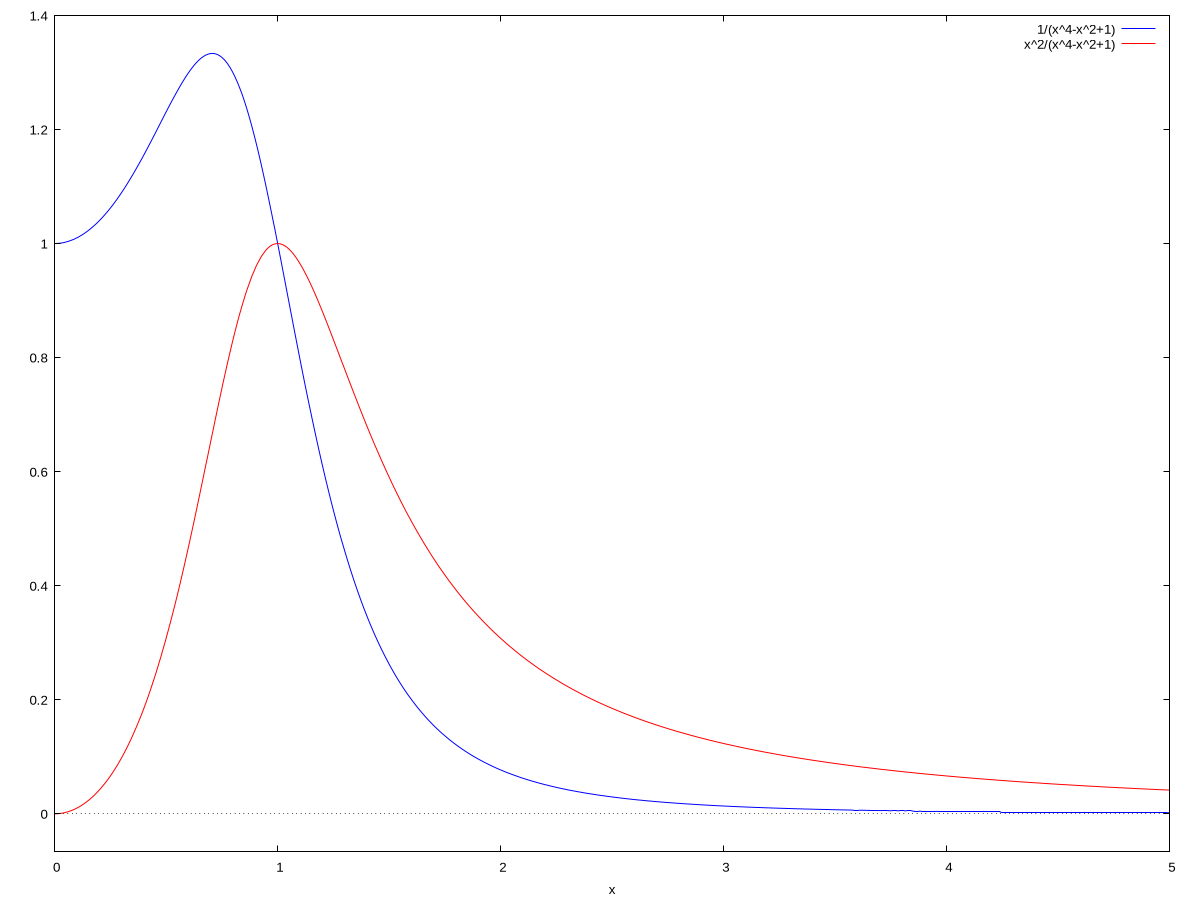
\includegraphics[scale=0.3]{images/2022-02-14_plot_1.png}
\end{figure}



%%% Local Variables:
%%% mode: latex
%%% TeX-master: "journal"
%%% End:
